\begin{figure}[ht]
	\begin{subfigure}[b]{0.32\linewidth}
		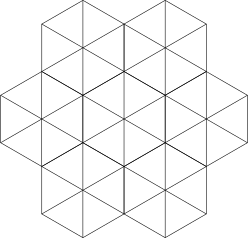
\includegraphics[width=\linewidth]
		{data/synthetic_meshes/hexagonal_tessellation_Dirac_delta_1_v31_f42_wireframe.png}
		\caption{$r=1$, wireframe}\label{fig:hex.a}
	\end{subfigure}
	\begin{subfigure}[b]{0.32\linewidth}
		\includegraphics[width=\linewidth]
		{data/synthetic_meshes/hexagonal_tessellation_Dirac_delta_1_v31_f42_funcvals_0iter_crop.png}
		\caption{$r=1$, $c=0$}\label{fig:hex.b}
	\end{subfigure}
	\begin{subfigure}[b]{0.32\linewidth}
		\includegraphics[width=\linewidth]
		{data/synthetic_meshes/hexagonal_tessellation_Dirac_delta_1_v31_f42_funcvals_2iter_crop.png}
		\caption{$r=1$, $c=2$}\label{fig:hex.c}
	\end{subfigure}

	\begin{subfigure}[b]{0.32\linewidth}
		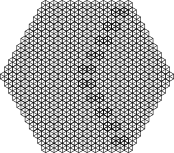
\includegraphics[width=\linewidth]
		{data/synthetic_meshes/hexagonal_tessellation_Dirac_delta_10_v1057_f1986_wireframe.png}
		\caption{$r=10$, wireframe}\label{fig:hex.d}
	\end{subfigure}
	\begin{subfigure}[b]{0.32\linewidth}
		\includegraphics[width=\linewidth]
		{data/synthetic_meshes/hexagonal_tessellation_Dirac_delta_10_v1057_f1986_funcvals_0iter_crop.png}
		\caption{$r=10$, $c=0$}\label{fig:hex.e}
	\end{subfigure}
	\begin{subfigure}[b]{0.32\linewidth}
		\includegraphics[width=\linewidth]
		{data/synthetic_meshes/hexagonal_tessellation_Dirac_delta_10_v1057_f1986_funcvals_200iter_crop.png}
		\caption{$r=10$, $c=200$}\label{fig:hex.f}
	\end{subfigure}
	\caption[Six Views Comparing Hexagonal Tessellations]{Comparison of two differently-sized, hexagonal tessellations, generated with parameters $r$ set to 1 and 10. (a) $r=1$ in wireframe, (b) $r=1$ colored by function value before convolving the filter, (c) $r=1$ colored by function value after convolving the filter once, (d) $r=10$ in wireframe, (e) $r=10$ colored by function value before convoving the filter, and (f) $r=10$ colored by function value after convolving the filter 200 times.}
	\label{fig:hex}
\end{figure}
